% !TeX root = RJwrapper.tex
\title{\pkg{penPHcure}: Variable Selection in Proportional Hazards Cure Model with Time-Varying Covariates}
\author{by Alessandro Beretta and C\'edric Heuchenne}

\maketitle

\abstract{
We describe the \CRANpkg{penPHcure} R package, which implements the semiparametric proportional-hazards (PH) cure model of \citet{Sy_Taylor_2000} extended to time-varying covariates and the variable selection technique based on its SCAD-penalized likelihood proposed by \citet{Beretta_Heuchenne_2019}. 
In survival analysis, cure models are a useful tool when a fraction of the population is likely to be immune from the event of interest.
They can separate the effects of certain factors on the probability of being susceptible and on the time until the occurrence of the event.
Moreover, the \pkg{penPHcure} package allows the user to simulate data from a PH cure model, where the event-times are generated on a continuous scale from a piecewise exponential distribution conditional on time-varying covariates, with a method similar to \citet{Hendry_2014}.
We present the results of a simulation study to assess the finite sample performance of the methodology and illustrate the functionalities of the \pkg{penPHcure} package using criminal recidivism data.
}




\section{Introduction}
In contrast to other statistical methods, survival analysis models are designed to model the time to an event of interest (e.g., death or occurrence of a disease in medical studies). 
A typical feature of time-to-event data is the presence of right censoring,
an incomplete information problem that arises when a subject is lost to follow-up or does not experience the event before the end of the study. 
In these cases, it is unknown whether the subject will eventually experience the event and when it will occur, given that it can occur.
The most common assumption of standard survival analysis models is that the whole population will sooner or later experience the event of interest.
However, in practice, this may not be the case because a fraction of the population may be immune (i.e., not susceptible) to this event.
\emph{Cure models}, also known as \emph{split population duration models} or \emph{limited-failure population models}, were developed to handle this kind of situation.
They allow us to investigate the effects of some covariates (e.g., type of treatment, stage of the tumor, sex, or age) on the probability to be susceptible to the event of interest (i.e., incidence), and on the survival time conditional on being susceptible (i.e., latency).

Originally, cure models were introduced in the medical literature by \citet{Boag_1949} and \citet{Berkson_Gage_1952}, but they have been used in several other disciplines during the years.
In reliability engineering, \citet{Meeker_1987} investigates the failure of solid-state electronic components (e.g., integrated circuits).
In social science, \citet{Schmidt_Witte_1989} investigate the timing of return to prison for a sample of prison releases, and they use it to make predictions of whether or not individuals return to prison.
In finance, \citet{Cole_Gunther_1995} analyze the determinants of commercial bank failures in the United States; in credit scoring, \citet{Tong_2012} predict defaults on a portfolio of UK personal loans. 
In political science, \citet{Svolik_2008} studies the likelihood that a democracy consolidates and the timing of authoritarian reversals in democracies that are not consolidated.
In marketing, \citet{Polo_2011} investigate the drivers of customer retention in a liberalizing market, using data for a sample of 650 consumers in the Spanish mobile phone industry.
In the literature, several variants of cure models have been proposed (see \citet{Amico_2018} for a comprehensive survey), which belong to two main families: mixture cure models and promotion time cure models.

In this article, we present the \pkg{penPHcure} package \citep{penPHcure}, which implements
the semiparametric proportional-hazards (PH) mixture cure model of \citet{Sy_Taylor_2000} extended to time-varying covariates, where the incidence and latency distributions are modeled by a logistic regression and a Cox’s PH model \citep{Cox_1972}, respectively.
The \pkg{penPHcure} package contains two main functions: \code{penpHcure}, to estimate the regression coefficients, their confidence intervals using the basic/percentile bootstrap method, and to perform variable selection using the SCAD-penalized likelihood technique proposed by \citet{Beretta_Heuchenne_2019}; and \code{penpHcure.simulate} to simulate data from a PH cure model, where the event-times are generated on a continuous scale from a piecewise exponential distribution conditional on time-varying covariates, using a method similar to the one described in \citet{Hendry_2014}.

At the time of writing this article, we are unaware of other R packages for estimation of semiparametric PH mixture cure models with time-varying covariates and, above all, that enable the user to perform variable selection. 
In the context of cure models for right-censored data, available R packages include: 
the \CRANpkg{flexsurvcure} package \citep{flexsurvcure} for estimation of parametric mixture and non-mixture cure models with time-invariant covariates using time-to-event distributions from the \CRANpkg{flexsurv} package \citep{flexsurv}; 
the \CRANpkg{nltm} package \citep{nltm} for estimation of the semiparametric PH cure model with time-invariant covariates of \citet{Tsodikov_2003_cure}, as well as other nonlinear transformation models for analyzing survival data using the method of \citet{Tsodikov_2003_general}; 
and the \CRANpkg{smcure} package \citep{smcure} for estimation of the semiparametric PH cure model and the accelerated failure time cure model with time-invariant covariates and the \CRANpkg{spduration} package \citep{spduration} that implements a parametric cure model with time-varying covariates using Weibull and Log-Logistic latency distributions. 
Compared to \code{spduration}, the \pkg{penPHcure} package has some advantages: the latency distribution is modeled by a more flexible semiparametric Cox's PH model; the response variable and the time to the event of interest are continuous; and, above all, it allows the user to simultaneously select variables and estimate their parameters using a variable selection technique based on SCAD penalties.


The remainder of this article is structured as follows: 
\begin{itemize}
	\item \textit{Methodology}. We present the PH cure model with time-varying covariates implemented in the \code{penPHcure} function when the argument \code{pen.type} is set equal to \code{"none"} (default);
	\begin{itemize}
		\item \textit{Variable selection}. We present the variable selection technique based on SCAD penalties implemented in the \code{penPHcure} function when \code{pen.type=="SCAD"};
		\item \textit{Data generation}. We describe the algorithm implemented in the \code{penPHcure.simulate} function, which generates data from a PH cure model with time-varying covariates.
	\end{itemize}
	\item \textit{Simulation study}. We analyze the finite sample performance of the PH cure model estimates and its variable selection technique implemented in the \code{penPHcure} function.
	\item \textit{An application to Criminal Recidivism data}. We provide an example of practical use of the \code{penPHcure} function to analyze a real data set.
\end{itemize}


\section{Methodology}

Let $Y$ be a Bernoulli random variable indicating whether an individual is susceptible ($Y=1$) or immune ($Y=0$) to the event of interest with probability $p=P(Y=1)$. Let $T$ be the time to event, defined only when $Y=1$. Assuming that a fraction of the population is immune to the event of interest, the marginal survival function of $T$ is defined as
$$S(t)=(1-p)+pS(t|Y=1),$$
where $p$ is the incidence (i.e., probability of being susceptible) and $S(t|Y=1)$ is the latency (i.e., survival function conditional on being susceptible).

The incidence is modeled by a logistic regression model:
$$p(\textbf{x})=P(Y=1|\mathbf{x})=\frac{\exp(\mathbf{x}'\textbf{b})}{1+\exp(\mathbf{x}'\textbf{b})},$$
where $\textbf{x}$ is a vector of time-fixed covariates (including the intercept) and $\mathbf{b}$ a vector of unknown coefficients. Whereas the latency is modeled by a Cox's PH model:
$$S(t|Y=1,\bar{\textbf{z}}(t))=\exp\left( - \int_0^t h_{0}(u)e^{\textbf{z}'(u)\boldsymbol{\beta} du}\right),$$ 
where $\textbf{z}(t)$ is a vector of time-varying covariates (we denote by $\bar{\textbf{z}}(t)$ the full history of the covariates up to time $t$), $\boldsymbol{\beta}$ is a vector of unknown coefficients, and $h_{0}(t)$ is an arbitrary baseline conditional hazard function. 

Let $\textbf{O}=\left\{ (t_{i},\delta_{i},\bar{\textbf{z}}_{i}(t_i),\textbf{x}_{i}) ; i=1,...,n \right \}$ denote the observed data, where $t_{i}$ is the event/censoring time and $\delta_{i}$ is the censoring indicator, which takes value 1 if $t_{i}$ is uncensored and 0 otherwise. 
Since we know that $y_i=1$ when $\delta_i=1$, but $y_i$ is unobserved when $\delta_i=0$, we can estimate the unknown parameters $\boldsymbol{\theta}=(\textbf{b},\boldsymbol{\beta},h_{0})$ using the Expectation-Maximization (EM) algorithm \citep{Dempster_1977}. The complete-data likelihood can be written as
\begin{equation}
\label{eq:comp_data_likelihood}
L_{C}\left(\textbf{b},\boldsymbol{\beta},h_{0}\right)=\underbrace{ \prod_{i=1}^{n}p(\textbf{x}_i)^{y_{i}}\left[1-p(\textbf{x}_i)\right]^{(1-y_{i})} }_{L_{1}(\textbf{b})} \times \underbrace{ \prod_{i=1}^{n}\left[h_{0}(t_{i})e^{\textbf{z}'_{i}(t_{i})\boldsymbol{\beta}}\right]^{\delta_{i}y_{i}}\left[e^{-\int_{0}^{t_i}h_{0}(u)e^{\textbf{z}'_{i}(u)\boldsymbol{\beta}}\ du}\right]^{y_{i}} }_{L_{2}(\boldsymbol{\beta},h_{0})},
\end{equation}
i.e., the product between the incidence component $L_{1}$ depending on a set of time-fixed covariates $\textbf{x}_i$, and the latency component $L_{2}$ depending on a set of time-varying covariates $\textbf{z}'_{i}(t)$.

Given some starting values $\boldsymbol{\theta}^{(0)}$, the $m$-th iteration of the EM algorithm consists of two steps:
\begin{description}
 \item [\textit{E step}.] Compute the expectation of the complete-data likelihood with respect to the conditional distribution of the $y_i$'s given the current parameter estimates $\hat{\boldsymbol{\theta}}^{(m-1)}$ and the observed data $\textbf{O}$.
 This expectation is obtained by replacing the $y_i$'s in \eqref{eq:comp_data_likelihood} by their expectation
$$\pi_{i}^{(m)}=E\left[Y_{i}\left|\hat{\boldsymbol{\theta}}^{(m-1)},\textbf{O}\right.\right]= \delta_i + (1-\delta_i) \frac{p(\textbf{x}_i)S(t|Y=1,\bar{\textbf{z}}_i(t))}{1-p(\textbf{x}_i)+p(\textbf{x}_i)S(t|Y=1,\bar{\textbf{z}}_i(t))}.$$
 Note that we removed the dependence of the theoretical functions on the estimated parameters to simplify the notation.
 \item [\textit{M step}.] Maximize the expected complete-data likelihood with respect to $\textbf{b}$, $\boldsymbol{\beta}$, and the function $h_0$. 
 Given $\boldsymbol{\pi}^{(m)}=\{\pi_{1}^{(m)},...,\pi_{n}^{(m)}\}$, the incidence component $L_{1}$ in \eqref{eq:comp_data_likelihood} is maximized 
 using the Newton-Raphson method as in the classical logistic regression model. Whereas the latency component $L_{2}$ in \eqref{eq:comp_data_likelihood} is maximized using a profile likelihood approach. The latter involves two steps: (i) the baseline conditional hazard function is estimated nonparametrically by
 \begin{equation}
 \label{eq:base_haz_est}
 \hat{h}_0(t) = \frac{1}{\left(t_{(j)}-t_{(j-1)}\right)\sum_{i\in R_{j}}\pi_{i}^{(m)}e^{\textbf{z}'_{i}(t_{(j)})\boldsymbol{\beta}}}, \hspace{0.2cm} \hbox{ for } t\in(t_{(j-1)},t_{(j)}],
 \end{equation}
 where $t_{(1)}\leq...\leq t_{(k)}$ are the $k$ ordered event times and $R_j$ is the risk set at $t_{(j)}^-$ (i.e., the set of all individuals who did not experience the event of interest and have not been censored just prior to time $t_{(j)}$);
 and then (ii) the function $h_0$ in $L_2$ is replaced by its estimator given in \eqref{eq:base_haz_est} to obtain the following partial likelihood, which does not depend on the function $h_0$ anymore,
 \begin{equation}
 \label{eq:partial_like}
 \tilde{L}_{2}\left(\boldsymbol{\beta}\left|\boldsymbol{\pi}_{i}^{(m)}\right.\right)= \prod_{j=1}^{k}\frac{e^{\textbf{z}_{i}(t_{(j)})\boldsymbol{\beta}}}{\sum_{i\in R_{j}}\pi_{i}^{(m)}e^{\textbf{z}'_{i}(t_{(j)})\boldsymbol{\beta}}}.
 \end{equation}
 Finally, the latency component is estimated by maximizing \eqref{eq:partial_like} with respect to $\boldsymbol{\beta}$.
 In case of tied event-times, \eqref{eq:base_haz_est} and \eqref{eq:partial_like} can be rewritten using the \citet{Breslow_1974} or \citet{Efron_1977} approximation as in the standard Cox's PH model.
\end{description}

The EM algorithm terminates whenever $\left\|\hat{\textbf{b}}^{(m)}-\hat{\textbf{b}}^{(m-1)}\right\|_2 < \epsilon$ and $\left\|\hat{\boldsymbol{\beta}}^{(m)}-\hat{\boldsymbol{\beta}}^{(m-1)}\right\|_2 < \epsilon$, where $\epsilon$ is a tolerance threshold (by default $10^{-6}$).



\subsection{Variable selection}

When the number of available covariates is large, fitting all possible subsets to find the most relevant covariates would be too time consuming.
\citet{Beretta_Heuchenne_2019} proposed a regularization method based on the maximization of a penalized version of the complete-data log-likelihood

$$\ell_C^P \left(\boldsymbol{\theta};\lambda_{1},\lambda_{2}\right) = \underbrace{\ell_1 \left(\textbf{b}\right) -n\sum_{j=2}^{q_1+1}p_{\lambda_{1}}\left(|b_{j}|\right)}_{\ell_1^P \left(\textbf{b};\lambda_{1}\right)} + \underbrace{\ell_2 \left(\boldsymbol{\beta},\textbf{h}_{0}\right) - n\sum_{l=1}^{q_2}p_{\lambda_{2}}\left(|\beta_{l}|\right)}_{\ell_2^P \left(\boldsymbol{\beta},\textbf{h}_{0};\lambda_{2}\right)},$$
where $\ell$ denotes a log-likelihood and $p_\lambda(.)$ a SCAD penalty function,
which role is to shrink the small coefficients toward zero. We assume that the $q_1$ and $q_2$ covariates in the incidence and latency component, respectively, have been standardized, such that the coefficients in $\mathbf{b}$ and $\boldsymbol{\beta}$ are on the same scale.
The Smoothly Clipped Absolute Deviation (SCAD) penalty function \citep{Fan_Li_2001} is given by
$$
p_{\lambda}(|\beta_{j}|)=\begin{cases}
\lambda|\beta_{j}|, & \textrm{if }|\beta_{j}|\leq\lambda\\
\frac{(a^{2}-1)\lambda^{2}-(|\beta_{j}|-a\lambda)^{2}}{2(a-1)}, & \textrm{if }\lambda<|\beta_{j}|\leq a\lambda\\
\frac{(a+1)\lambda^{2}}{2}, & \textrm{if }|\beta_{j}|>a\lambda
\end{cases},\label{eq:SCAD_penalty}
$$
for some $a>2$ and $\lambda>0$.  
As explained by \citet{Fan_Li_2001,Fan_Li_2002} in the context of linear regression, generalized linear models, Cox's PH model, and frailty models, the SCAD estimator has three desirable properties: unbiasedness (do not penalize to much large coefficients), sparsity, and continuity. 
Moreover, with a proper choice of the tuning parameters $(\lambda,a)$, it also possesses what is known as the ``oracle property'', meaning that the SCAD estimator is asymptotically equivalent to the oracle estimator (i.e., an estimator with only the relevant variables with nonzero coefficients). 

For fixed values of the tuning parameters $(\lambda_1,\lambda_2,a_1,a_2)$, estimates of $\boldsymbol{\theta}$ can be obtained using an EM algorithm close to the one described in the previous section. 
The only difference lies in the M-step. Given that the penalized log-likelihoods $\ell_1^P \left(\textbf{b};\lambda_{1}\right)$ and $\tilde{\ell}_2^P \left(\boldsymbol{\beta};\lambda_{2}\right)$, where $\tilde{\ell}_2^P \left(\boldsymbol{\beta};\lambda_{2}\right)$ is the logarithm of (\ref{eq:partial_like}), are non-concave and non-differentiable at the origin, $\textbf{b}$ and $\boldsymbol{\beta}$ are now estimated using the MM algorithm of \citet{Hunter_Li_2005} based on a perturbed Local Quadratic Approximation (LQA) of the penalty function. By default, when the argument \code{pen.type} of the function \code{penPHcure} is set equal to \code{"SCAD"}, the initial values for $\mathbf{b}$ and $\boldsymbol{\beta}$ are vectors with all elements equal to zero. Otherwise, the user can specify other values (e.g., the estimated coefficients of the model with all covariates) using the argument \code{SV}.

Regarding the choice of the tuning parameters, following the suggestion of \citet{Fan_Li_2001}, we keep $a_1=a_2=3.7$, and given a set of possible values for $(\lambda_1,\lambda_2)$, we select the ones that minimize the following Akaike (AIC) or Bayesian (BIC) Information Criteria: 
$$\mathrm{AIC}\left(\lambda_{1},\lambda_{2}\right)=-2\ell\left(\hat{\boldsymbol{\theta}}_{\lambda_{1},\lambda_{2}}\right) + 2 \nu; \ \hbox{ and}$$
$$\mathrm{BIC}\left(\lambda_{1},\lambda_{2}\right)=-2\ell\left(\hat{\boldsymbol{\theta}}_{\lambda_{1},\lambda_{2}}\right) + \ln(n) \nu,$$
where $\ell\left(\hat{\boldsymbol{\theta}}_{\lambda_{1},\lambda_{2}}\right)$ is the observed data log-likelihood evaluated at the penalized MLE $\hat{\boldsymbol{\theta}}_{\lambda_{1},\lambda_{2}}$ and $\nu$ is the number of nonzero coefficients, identified as the number of coefficients with an absolute value greater than a given threshold (by default $10^{-6}$).






\subsection{Data generation}
Let $\mathbf{S}=\{s_1,s_2,...,s_J\}$ be a partition of the time scale forming $J+1$ intervals $(0,s_1]$, $(s_1,s_2]$, $...$, $(s_{J-1},s_J]$, $(s_{J},\infty]$.
Define a vector of time-varying covariates piecewise constant in each interval: $\mathbf{z}(t)=\mathbf{z}_j$, for $t\in(s_{j-1},s_j]$. 
Consider a transformation $g$, such that $g(0)=0$, $g(t)$ is strictly increasing for $t>0$, and $g^{-1}(t)$ is differentiable.
In the implementation of the \code{penPHcure.simulate} function, we use $g(t)=t^{1/\gamma}$, where the parameter $\gamma$ can be specified by the user via the argument \code{gamma}, which by default is equal to 1.
According to \citet{Hendry_2014}, if we generate a random variable $V$ as a piecewise exponential distribution with density function given by
$$f_V(t) = \prod_{l=1}^{j-1} \exp\{-\lambda_l[g^{-1}(s_l)-g^{-1}(s_{l-1})]\} \lambda_j \exp\{-\lambda_j[t-g^{-1}(s_{j-1})]\}, \ \ \hbox{for } t\in(g^{-1}(s_{j-1}),g^{-1}(s_j)],$$
where $\lambda_j=\exp(\mathbf{z}_j'\boldsymbol{\beta})$ is the constant hazard in the interval $(g^{-1}(s_{j-1}),g^{-1}(s_{j})]$, then $g(V)$ follows a Cox's PH model with time-varying covariates with a baseline hazard function given by $h_0(t)=\frac{d}{dt}[g^{-1}(t)]$.
This method is part of the algorithm implemented in the \code{penPHcure.simulate} function to simulate data from a PH cure model with time-varying covariates (see Table \ref{algo:datagen} for a detailed description).

\algnewcommand\Or{\textbf{or} }
\begin{table}[ht]
  \begin{algorithmic}
  \hrule
    \Require $N$, sample size; $\mathbf{S}$, partition of the time scale; $g(t)$, variable transformation; $\mathbf{b}$, incidence coefficients; $\boldsymbol{\beta}$, latency coefficients.
  \hrule
    \For{$i = 1,...,N$}
      \State 1. Generate a vector $\mathbf{x}_i$ from an arbitrary distribution; %\Comment{Time-invariant covariates}
      \State 2. Generate $y_i$ from a Bernoulli distribution with probability $p(\mathbf{x}_i)$; %\Comment{Susceptibility indicator} 
      \State 3. Generate $\mathbf{z}_{i}=\{\mathbf{z}_{i,1},\mathbf{z}_{i,2},...\mathbf{z}_{i,J}\}$ from an arbitrary distribution; %\Comment{Time-varying covariates}
      \State 4. Generate $v_i$ from a piecewise exponential distribution with density $f_V(t)$;
      \State 5. Compute $w_i = g(v_i)$ ; %\Comment{Event time}
      \State 6. Generate $c_i$ from an arbitrary distribution; %\Comment{Censoring time}
      \If{$y_i=0$ \Or $w_i>c_i$} %\Comment{If not susceptible}
        \State $t_i = c_i$;
        \State $\delta_i=0$;  
      \Else
        \State $t_i = w_i$;
        \State $\delta_i=1$;
      \EndIf
    \EndFor \\
    \Return $\{(t_i,\delta_i,\mathbf{z}_i,\mathbf{x}_i); i=1,...,N\}$
  \hrule
  \end{algorithmic}
\caption{Data generation algorithm: PH cure model with time-varying covariates}
\label{algo:datagen}
\end{table}










\section{Simulation study} 

In this section, we present the results of a simulation study conducted to assess the finite sample performance of the PH cure model estimation and its variable selection technique implemented in the \code{penPHcure} function. 
The event-times follow a Cox's PH model with baseline hazard function $h_0(t)=3t^2$ and 8 time-varying covariates. These covariates are constant within $J=30$ equally-spaced intervals $(0,s_1]$, $(s_1,s_2]$, $...$, $(s_{J-1},s_J]$, where $s_1=0.2$ and $s_J=6$.
They follow a multivariate normal distribution $\mathbf{z}_{i,j}\sim N(\mathbf{0},\boldsymbol{\varSigma})$, where $\varSigma_{p,q}=0.5^{|p-q|}$, for $p,q=1,...,8$.
The censoring times follow an exponential distribution truncated above $6$ and with parameter $\lambda_C$. The cure indicators are generated from a logistic regression model with 8 time-fixed covariates that follow a multivariate normal distribution $\mathbf{x}_{i}\sim N(\mathbf{0},\boldsymbol{\varSigma})$, where $\varSigma_{p,q}=0.5^{|p-q|}$, for $p,q=1,...,8$. Finally, the regression coefficients vectors are set equal to $\boldsymbol{\beta}_0=(-0.7,0,1,0,-0.5,0.75,0,0)'$ and $\mathbf{b}_0=(b_0,1.5,0,-0.75,0,-1.5,0,0.75,0)'$.

We consider 6 simulation settings, with different levels of censoring and proportions of non-susceptible individuals (expressed as a fraction of the sample size), depending on different values of $b_0$ and $\lambda_C$ (see Table~\ref{table:sim_settings}).
For each of these settings, we generated 500 replications using the \code{penPHcure.simulate} function for different sample sizes $N=\{250,500,1000\}$.
Then, for all simulated datasets, we use the \code{penPHcure} function to (i) fit a standard PH cure model with all covariates (FULL), (ii) fit a standard PH cure model with the covariates associated to the non-zero coefficients only (ORACLE), and (iii) to perform variable selection using the regularization method with SCAD penalties and tuning parameters chosen according to the BIC criterion.
The possible values of the tuning parameters $(\lambda_1,\lambda_2)$ are obtained with the function \code{exp(seq(-6, -1, length.out = 10))}, whereas $(a_1,a_2)$ are kept equal to $3.7$.
Furthermore, we use the \code{coxph} function in the \CRANpkg{survival} package \citep{survival} to fit the classical Cox's PH model with the covariates associated to the non-zero coefficients only (COX).

\begin{table}[ht]
\small
\begin{center}
\begin{tabular}{cccc}
\toprule
\textbf{Censoring} & \textbf{Cure} & $\lambda_C$ & $b_0$ \\
\midrule
Low (40\%) & High (30\%) & 0.02 & 1.45 \\
Low (40\%) & Medium (20\%) & 0.3 & 2.35 \\
Medium (60\%) & High (45\%) & 0.35 & 0.35 \\
Medium (60\%) & Medium (30\%) & 0.75 & 1.45 \\
High (80\%) & High (60\%) & 0.95 & -0.7  \\
High (80\%) & Medium (40\%) & 1.55 & 0.7 \\
\bottomrule
\end{tabular}
\end{center}
\caption{Simulation settings (censoring and cure are expressed as fractions of all individuals).}
\label{table:sim_settings}
\end{table}

The performance is measured in terms of Mean Estimation Error (MEE) and average number of correct and incorrect zeros identified by the variable selection technique (SCAD). 
In particular, the estimation error for the incidence component is computed as $E\left[ \left( \hat{p}(\mathbf{x}) - p_0(\mathbf{x}) \right)^2 \right]$, where $\hat{p}(\mathbf{x})$ and $p_0(\mathbf{x})$ are the estimated and true probabilities of being susceptible. 
Whereas the estimation error for the latency component is computed as $E\left[ \left( \hat{S}(T|Y=1)  - S_0(T|Y=1) \right)^2 \right]$, where $\hat{S}(T|Y=1)$ and $S_0(T|Y=1)$ are the estimated and true survival functions conditional on being susceptible.


In \Cref{figure:errors_CURE,figure:errors_SURV}, we provide the MEEs for the incidence and latency components, respectively, while in \Cref{figure:zeros_SCAD}, we provide the average number of correct and incorrect zeros.
From those figures, we can see that the PH cure model estimation and its variable selection technique implemented in the \code{penPHcure} function perform reasonably well. 
For an increase of the sample size or a decrease of the level of censoring, the MEE decreases, and the number of correct (resp. incorrect) zeros converges to 4 (resp. 0).
The MEEs of the ORACLE model are always the lowest ones, but we notice that the ones of the SCAD method tend towards them as the sample size increases.
It is important to note that, for a fixed level of censoring, we observe higher MEEs in the case of a lower fraction of cured individuals. 
The worst results are obtained in situations of high censoring and low cure rates, but it is enough to increase the sample size to obtain better results.
This is evidence of the fact that a cure model should always be applied to data with a sufficient number of non-susceptible individuals.
Last but not the least important, we note that the use of the classical Cox's PH model (COX) leads to very high errors. 
This was expected since the model is wrongly specified as it ignores the existence of cured subjects.


\begin{figure}[hb!]
  \centering
  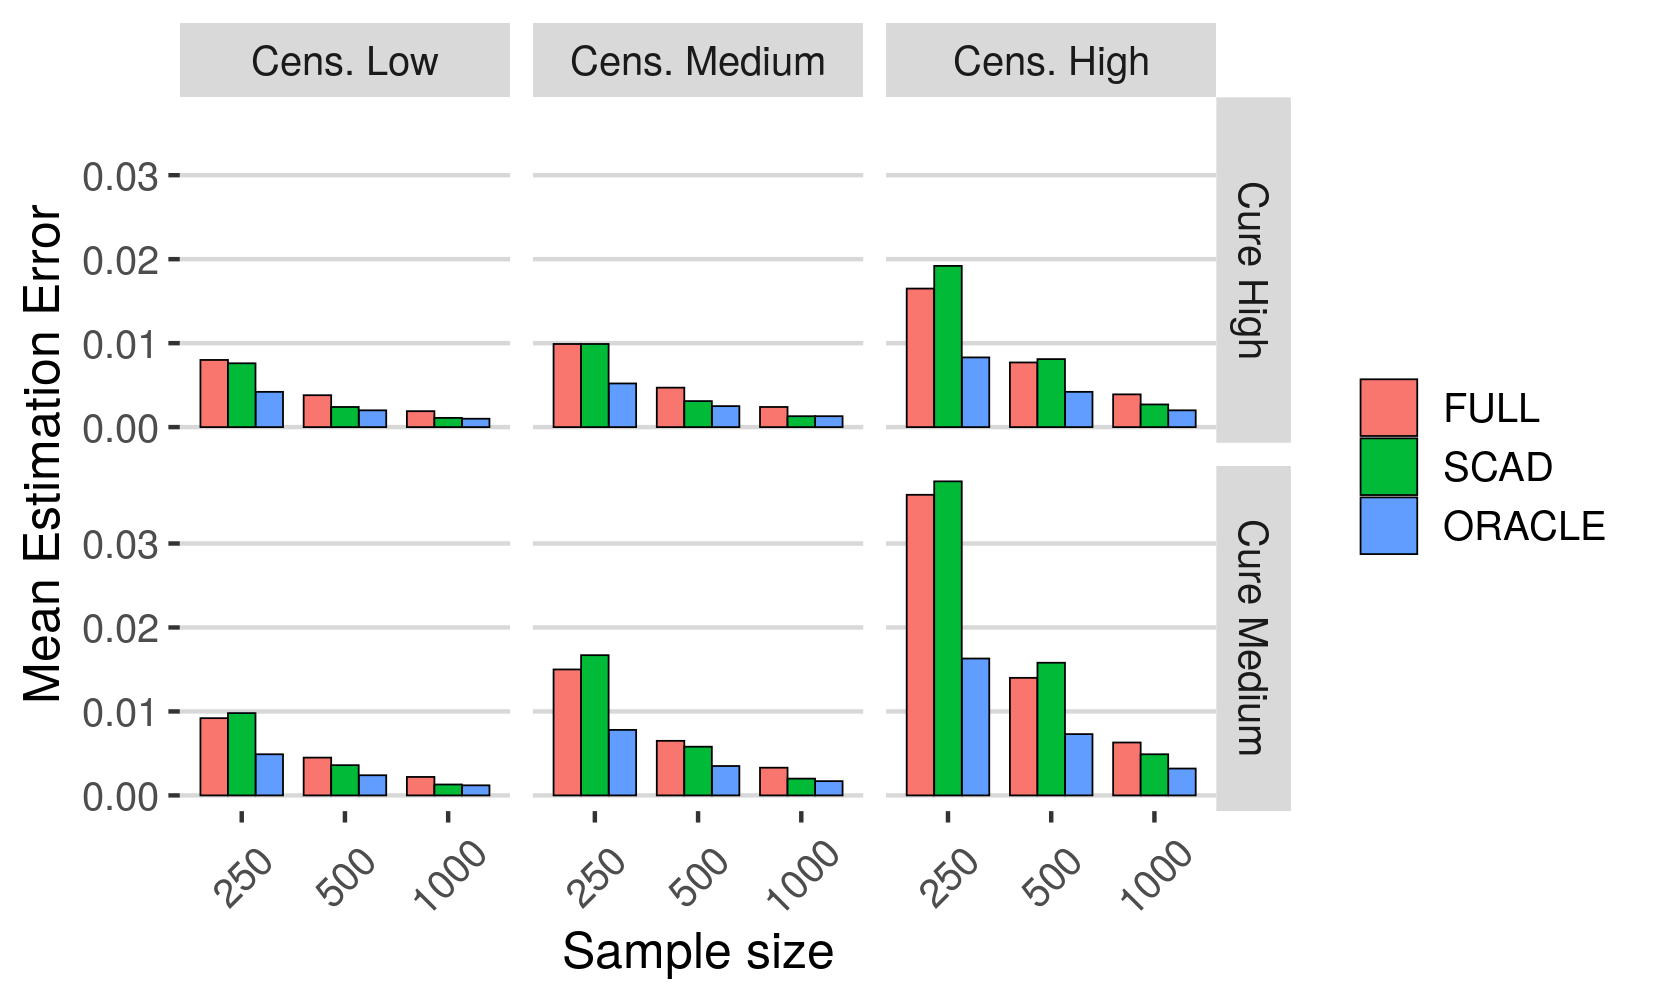
\includegraphics[scale=0.83]{fig_errors_CURE.png}
  \caption{Results of the simulations: mean estimation errors (incidence component).}
  \label{figure:errors_CURE}
\end{figure}


\begin{figure}[hb!]
  \centering
  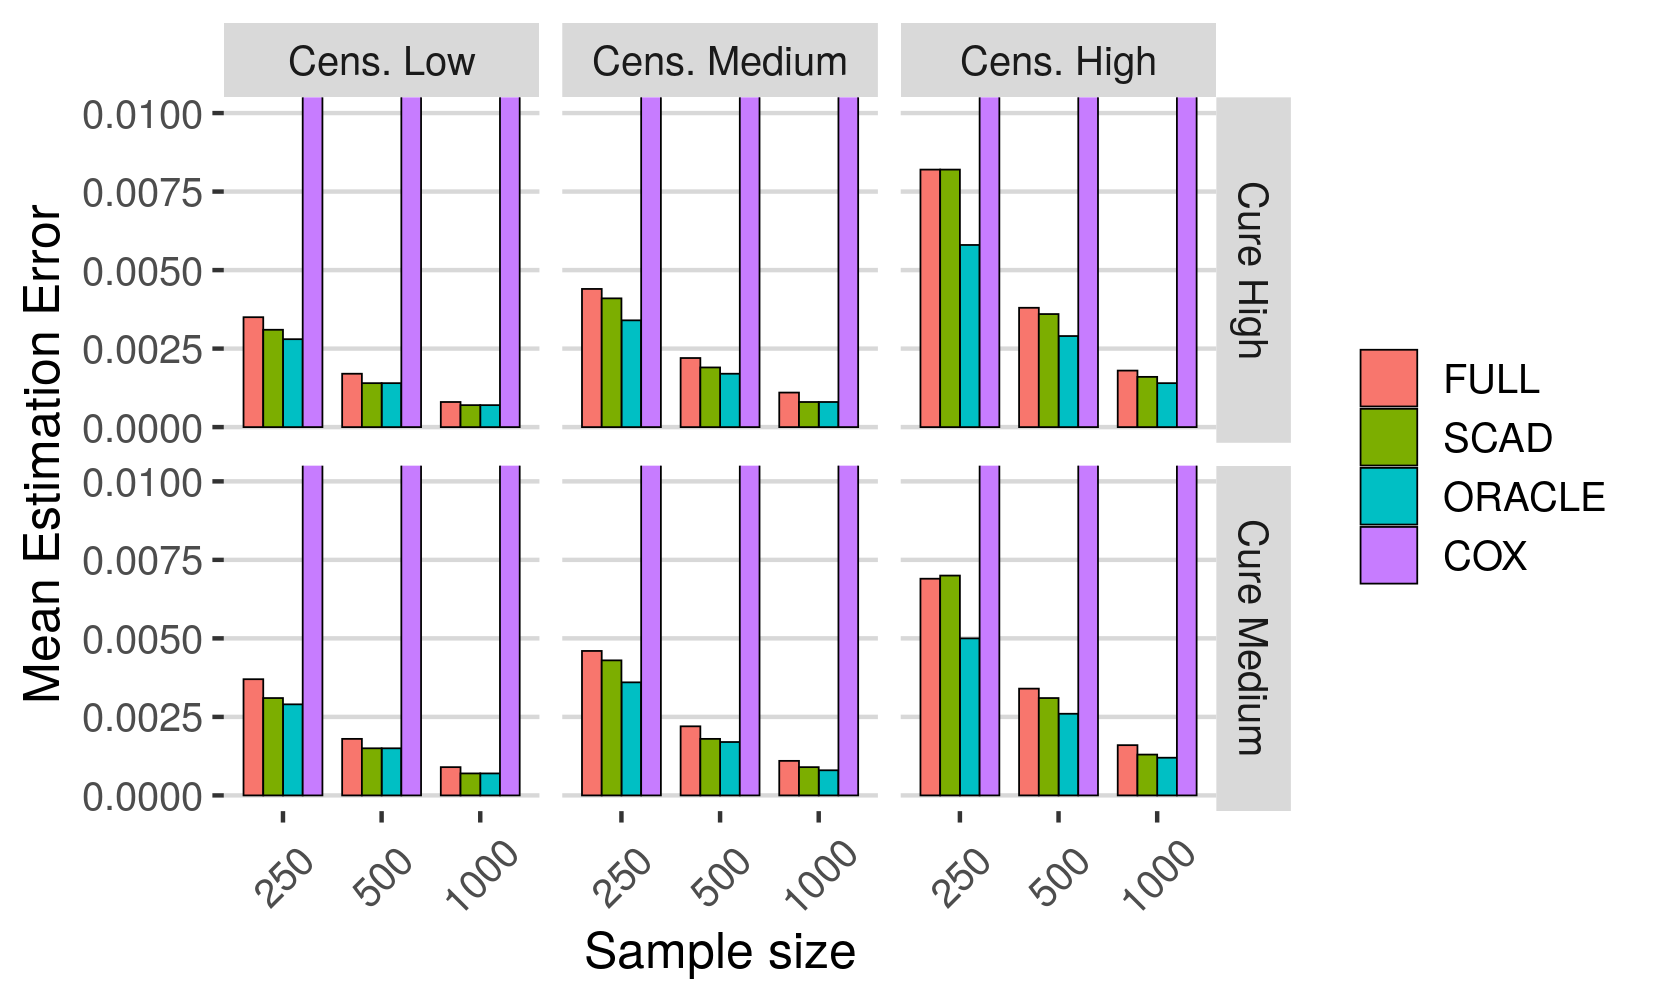
\includegraphics[scale=0.83]{fig_errors_SURV.png}
  \caption{Results of the simulations: mean estimation errors (latency component).}
  \label{figure:errors_SURV}
\end{figure}

\begin{figure}[hb!]
  \centering
  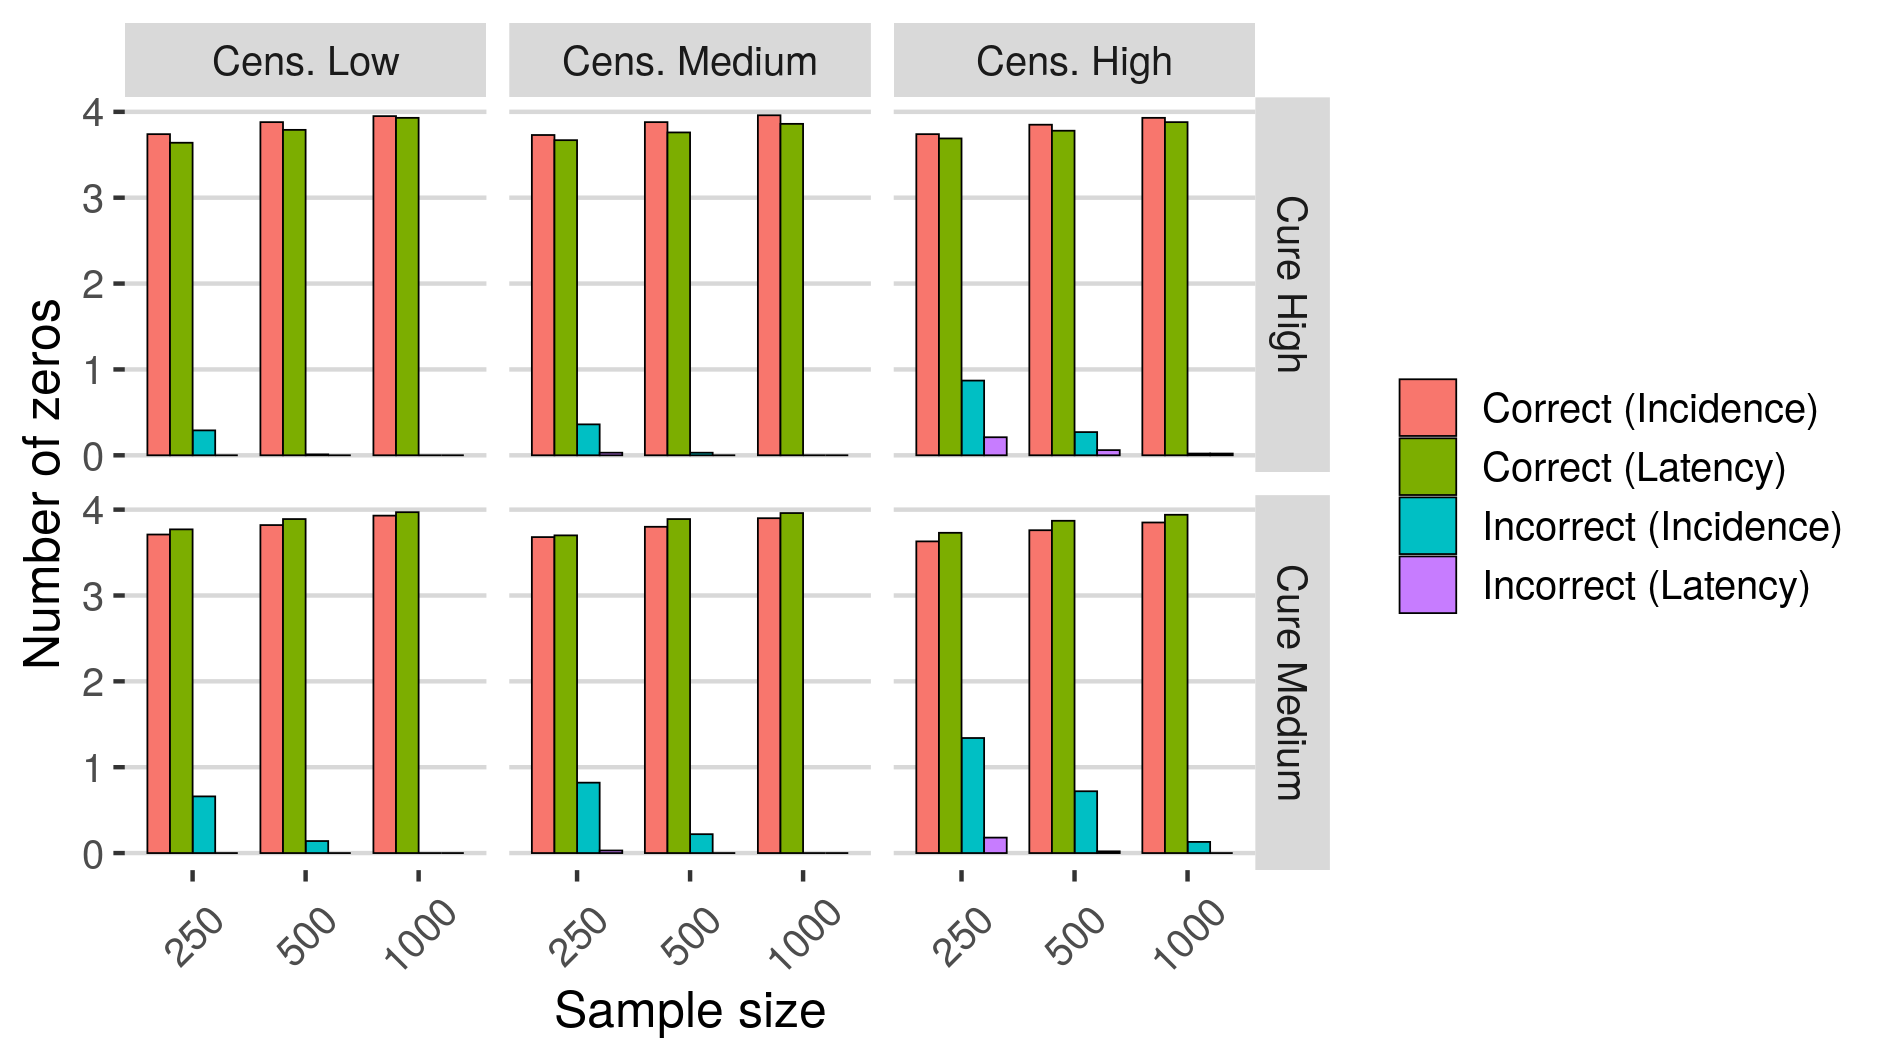
\includegraphics[scale=0.83]{fig_zeros_SCAD.png}
  \caption{Results of the simulations: average number of correct/incorrect zeros identified by the variable selection technique (SCAD).}
  \label{figure:zeros_SCAD}
\end{figure}


Finally, in Table~\ref{table:res_sim_cov_prob}, we also present the coverage probabilities of the estimated 95\% confidence intervals for the ORACLE model using the basic and percentile bootstrap methods with 500 resamples. In most cases, the basic bootstrap method outperforms the percentile bootstrap method, especially for the smallest sample sizes, with coverage probabilities closer to the 95\% nominal level. 


The R code used to obtain the results in \Cref{figure:errors_CURE,figure:errors_SURV,figure:zeros_SCAD} (resp. Table~\ref{table:res_sim_cov_prob}) are provided in Section 2 (resp. Section 3) of the supplementary material (\file{beretta-heuchenne.R}). Moreover, in the file \file{beretta-heuchenne-suppl.pdf}, we provide a table with all the results contained in \Cref{figure:errors_CURE,figure:errors_SURV,figure:zeros_SCAD}.



 \FloatBarrier

{\footnotesize
\begin{longtable}{cccc|ccccc|cccc}
\toprule
cens  & cure  & N & Method  & $b_0$ & $b_1$ & $b_2$ & $b_3$ & $b_4$ & $\beta_1$ & $\beta_2$ & $\beta_3$ & $\beta_4$ \\
\midrule
0.40 & 0.30 & 250 & basic & 0.97 & 0.97 & 0.98 & 0.97 & 0.97 & 0.96 & 0.97 & 0.96 & 0.94 \\ 
   &  &  & perc & 0.9 & 0.91 & 0.94 & 0.91 & 0.94 & 0.93 & 0.94 & 0.95 & 0.94 \\ 
   &  & 500 & basic & 0.97 & 0.95 & 0.95 & 0.94 & 0.96 & 0.96 & 0.96 & 0.96 & 0.96 \\ 
   &  &  & perc & 0.91 & 0.91 & 0.94 & 0.92 & 0.94 & 0.94 & 0.91 & 0.95 & 0.95 \\ 
   &  & 1000 & basic & 0.95 & 0.96 & 0.95 & 0.97 & 0.97 & 0.93 & 0.95 & 0.95 & 0.96 \\ 
   &  &  & perc & 0.94 & 0.94 & 0.93 & 0.95 & 0.97 & 0.93 & 0.95 & 0.95 & 0.95 \\ 
\midrule
  0.40 & 0.20 & 250 & basic & 0.95 & 0.96 & 0.99 & 0.96 & 0.97 & 0.96 & 0.97 & 0.97 & 0.96 \\ 
   &  &  & perc & 0.89 & 0.9 & 0.94 & 0.91 & 0.93 & 0.94 & 0.96 & 0.96 & 0.96 \\ 
   &  & 500 & basic & 0.98 & 0.97 & 0.97 & 0.97 & 0.98 & 0.95 & 0.96 & 0.96 & 0.96 \\ 
   &  &  & perc & 0.93 & 0.94 & 0.94 & 0.94 & 0.94 & 0.94 & 0.94 & 0.93 & 0.93 \\ 
   &  & 1000 & basic & 0.97 & 0.96 & 0.96 & 0.95 & 0.95 & 0.94 & 0.93 & 0.96 & 0.95 \\ 
   &  &  & perc & 0.95 & 0.94 & 0.94 & 0.93 & 0.94 & 0.94 & 0.94 & 0.96 & 0.95 \\ 
\midrule
  0.60 & 0.45 & 250 & basic & 0.98 & 0.95 & 0.96 & 0.96 & 0.97 & 0.98 & 0.98 & 0.97 & 0.97 \\ 
   &  &  & perc & 0.95 & 0.91 & 0.93 & 0.93 & 0.94 & 0.93 & 0.94 & 0.94 & 0.94 \\ 
   &  & 500 & basic & 0.98 & 0.95 & 0.94 & 0.97 & 0.96 & 0.94 & 0.94 & 0.96 & 0.95 \\ 
   &  &  & perc & 0.96 & 0.93 & 0.94 & 0.92 & 0.93 & 0.94 & 0.92 & 0.95 & 0.95 \\ 
   &  & 1000 & basic & 0.95 & 0.96 & 0.96 & 0.95 & 0.95 & 0.95 & 0.94 & 0.93 & 0.95 \\ 
   &  &  & perc & 0.95 & 0.94 & 0.94 & 0.93 & 0.94 & 0.94 & 0.92 & 0.94 & 0.93 \\ 
\midrule
  0.60 & 0.30 & 250 & basic & 0.96 & 0.94 & 0.98 & 0.94 & 0.99 & 0.97 & 0.96 & 0.96 & 0.96 \\ 
   &  &  & perc & 0.89 & 0.9 & 0.91 & 0.89 & 0.93 & 0.94 & 0.94 & 0.95 & 0.95 \\ 
   &  & 500 & basic & 0.96 & 0.97 & 0.98 & 0.95 & 0.97 & 0.96 & 0.96 & 0.95 & 0.95 \\ 
   &  &  & perc & 0.94 & 0.91 & 0.94 & 0.93 & 0.93 & 0.95 & 0.96 & 0.95 & 0.95 \\ 
   &  & 1000 & basic & 0.96 & 0.96 & 0.96 & 0.95 & 0.96 & 0.96 & 0.95 & 0.95 & 0.96 \\ 
   &  &  & perc & 0.95 & 0.94 & 0.94 & 0.92 & 0.94 & 0.94 & 0.94 & 0.94 & 0.95 \\ 
\midrule
  0.80 & 0.60 & 250 & basic & 0.99 & 0.97 & 0.98 & 0.97 & 0.97 & 0.97 & 0.96 & 0.97 & 0.97 \\ 
   &  &  & perc & 0.94 & 0.91 & 0.92 & 0.91 & 0.92 & 0.94 & 0.92 & 0.96 & 0.94 \\ 
   &  & 500 & basic & 0.98 & 0.95 & 0.97 & 0.95 & 0.97 & 0.97 & 0.96 & 0.98 & 0.98 \\ 
   &  &  & perc & 0.94 & 0.93 & 0.95 & 0.93 & 0.94 & 0.95 & 0.94 & 0.95 & 0.96 \\ 
   &  & 1000 & basic & 0.96 & 0.95 & 0.96 & 0.94 & 0.96 & 0.96 & 0.95 & 0.94 & 0.96 \\ 
   &  &  & perc & 0.93 & 0.95 & 0.94 & 0.93 & 0.95 & 0.95 & 0.94 & 0.93 & 0.93 \\ 
\midrule
  0.80 & 0.40 & 250 & basic & 0.98 & 0.95 & 0.99 & 0.98 & 1 & 0.97 & 0.96 & 0.99 & 0.99 \\ 
   &  &  & perc & 0.92 & 0.88 & 0.91 & 0.91 & 0.93 & 0.95 & 0.93 & 0.97 & 0.95 \\ 
   &  & 500 & basic & 0.97 & 0.95 & 0.97 & 0.96 & 0.98 & 0.96 & 0.96 & 0.97 & 0.96 \\ 
   &  &  & perc & 0.94 & 0.9 & 0.93 & 0.91 & 0.93 & 0.94 & 0.94 & 0.96 & 0.94 \\ 
   &  & 1000 & basic & 0.96 & 0.96 & 0.97 & 0.95 & 0.95 & 0.98 & 0.95 & 0.93 & 0.96 \\ 
   &  &  & perc & 0.96 & 0.95 & 0.95 & 0.94 & 0.93 & 0.94 & 0.94 & 0.93 & 0.93 \\ 
\bottomrule
\caption{Results of the simulations: coverage probabilities.} 
\label{table:res_sim_cov_prob}
\end{longtable}
}




\section{An application to Criminal Recidivism data}

In this section, we illustrate the use of the \pkg{penPHcure} R package using a Criminal Recidivism dataset, which contains a sample of 432 inmates released from Maryland state prisons and followed for one year after release \citep{Rossi_1980}. The aim of this study was to investigate the relationship between the time to first arrest after release and some covariates observed during the follow-up period. In particular, to study the effect of providing financial aid at the moment of release.  
The original source of the data is the \code{Rossi} dataset in the \CRANpkg{RcmdrPlugin.survival} package \citep{Fox_Carvalo_2012}, which has been converted into a counting process format and included in the \pkg{penPHcure} package.

Let us load and illustrate the dataset:
\begin{example}
> library(penPHcure)
> data("cpRossi", package = "penPHcure")
> head(cpRossi)
  id tstart tstop arrest fin age  race wexp mar paro prio educ emp
1  1      0    20    yes  no  27 black   no  no  yes    3    3  no
2  2      0     9     no  no  18 black   no  no  yes    8    4  no
3  2      9    14     no  no  18 black   no  no  yes    8    4 yes
4  2     14    17    yes  no  18 black   no  no  yes    8    4  no
5  3      0    16     no  no  19 other  yes  no  yes   13    3  no
6  3     16    17     no  no  19 other  yes  no  yes   13    3 yes
> str(cpRossi)
'data.frame': 1405 obs. of  13 variables:
 $ id    : int  1 2 2 2 3 3 3 4 4 4 ...
 $ tstart: int  0 0 9 14 0 16 17 0 4 21 ...
 $ tstop : int  20 9 14 17 16 17 25 4 21 31 ...
 $ arrest: Factor w/ 2 levels "no","yes": 2 1 1 2 1 1 2 1 1 1 ...
 $ fin   : Factor w/ 2 levels "no","yes": 1 1 1 1 1 1 1 2 2 2 ...
 $ age   : int  27 18 18 18 19 19 19 23 23 23 ...
 $ race  : Factor w/ 2 levels "black","other": 1 1 1 1 2 2 2 1 1 1 ...
 $ wexp  : Factor w/ 2 levels "no","yes": 1 1 1 1 2 2 2 2 2 2 ...
 $ mar   : Factor w/ 2 levels "yes","no": 2 2 2 2 2 2 2 1 1 1 ...
 $ paro  : Factor w/ 2 levels "no","yes": 2 2 2 2 2 2 2 2 2 2 ...
 $ prio  : int  3 8 8 8 13 13 13 1 1 1 ...
 $ educ  : Factor w/ 3 levels "3","4","5": 1 2 2 2 1 1 1 3 3 3 ...
 $ emp   : Factor w/ 2 levels "no","yes": 1 1 2 1 1 2 1 1 2 1 ...
\end{example}

The object \code{cpRossi} is a \code{data.frame} in counting process format with 1405 observations for 432 individuals on 13 variables.
The \code{id} variable provides the unique identification number for every individual in the study. The variables \code{tstart} and \code{tstop} denote the time interval of the observation (measured in weeks). The variable \code{arrest} denotes whether the individual has been arrested during the 1-year follow-up period. The remaining explanatory variables are described hereafter.
\begin{itemize}
  \item \code{fin}. Financial aid received after release: \code{yes} or \code{no};
  \item \code{age}. Age in years at the time of release;
  \item \code{race}. Race of the individual: \code{black} or \code{other};
  \item \code{wexp}. Full-time work experience before incarceration:  \code{yes} or \code{no};
  \item \code{mar}. Married at the time of release: \code{yes} or \code{no};
  \item \code{paro}. Released on parole: \code{yes} or \code{no};
  \item \code{prio}. Number of convictions prior to incarceration;
  \item \code{educ}. Level of education: <=9th degree (``3''), 10th or 11th degree (``4''), or >=12th degree (``5'');
  \item \code{emp}. Working full time during the observed time interval: \code{yes} or \code{no}. This is the only variable which is varying over time (e.g., the individual with \code{id = 2} did not work full time during the first 9 weeks after release, then he did for 5 weeks, and, finally, he has been arrested after 3 weeks without working full time).
\end{itemize}

Using the \code{penPHcure} function, by default, we can fit the standard PH cure model.
First, we use a formula object with the response on the left of the tilde operator and the explanatory variables to be included in the latency component on the right.
The response is a survival object returned by the \code{Surv(tstart,tstop,arrest)} function.
Then, using the argument \code{cureform}, we specify the explanatory variables to be included in the incidence component.
By default, these covariates are set equal to the last observation, but in this case, we set the argument \code{which.X = "mean"} to compute the time-weighted average over the full history.
Finally, setting the argument \code{inference = TRUE}, we conduct inference about the parameter estimates via bootstrapping (by default, 100 bootstrap resamples). The user can increase/decrease the number of bootstrap resamples with the argument \code{nboot}. 

\begin{example}
> set.seed(123) # for reproducibility
> fit <- penPHcure(Surv(tstart,tstop,arrest)~fin+age+race+wexp+mar+paro+prio+educ+emp,
+                  cureform = ~fin+age+race+wexp+mar+paro+prio+educ+emp,
+                  data = cpRossi,which.X = "mean",inference = TRUE)

Initializing PH cure model with time-varying covariates...

Number of individuals: 432
Censoring proportion: 0.736
Tied failure times: TRUE
Number of unique failure times: 49
Number of covariates in the survival component: 10
Number of covariates in the cure component: 10

Checking starting values...

Fitting standard PH cure model with time-varying covariates... Please wait...

Performing inference via bootstrapping... Please wait ...
  |==============================================================================| 100%
DONE!
\end{example}

This call to the \code{penPHcure} function returned an object of class \code{"PHcure"}, and we can print a summary of the results using the \code{summary} method.
By default, confidence intervals are computed using the basic bootstrap method (the alternative is percentile bootstrap) and a confidence level of 95\%.
In order to control these features, the user can provide the arguments \code{conf.int} and \code{conf.int.level}, respectively.

\begin{example}
> summary(fit)

------------------------------------------------------
+++   PH cure model with time-varying covariates   +++
------------------------------------------------------
Sample size: 432
Censoring proportion: 0.7361111
Number of unique event times: 49
Tied failure times: TRUE

log-likelihood:  -643.65 

------------------------------------------------------
+++     Cure (incidence) coefficient estimates     +++
+++          and 95% confidence intervals *        +++
------------------------------------------------------
             Estimate       2.5%     97.5%
(Intercept)  1.136709 -34.041743  9.769052
finyes      -0.455199  -2.299870 12.188817
age         -0.067715  -0.382429  0.413001
raceother   -0.100950  -2.988104 35.336024
wexpyes      0.251663  -3.257339  2.193371
marno        0.261947 -15.041406 35.102574
paroyes     -0.041289  -3.156395  1.659637
prio         0.068443  -0.285553  0.237089
educ4       -0.570782  -2.614311  2.532353
educ5       -1.163257 -39.473732 34.360612
empyes      -0.860659  -3.299354  1.216299

------------------------------------------------------
+++    Survival (latency) coefficient estimates    +++
+++          and 95% confidence intervals *        +++
------------------------------------------------------
           Estimate      2.5%     97.5%
finyes     0.062630 -1.427436  1.446067
age        0.046192 -0.067209  0.176043
raceother -0.759985 -2.770654  0.720247
wexpyes   -0.552549 -1.672866  0.576657
marno      0.123655 -2.327914  1.600195
paroyes    0.040388 -0.816177  1.110058
prio       0.048407 -0.107942  0.195763
educ4      0.588156 -0.545885  1.881803
educ5      0.838098 -2.527512  5.118107
empyes    -1.431782 -1.980471 -0.781978

------------------------------------------------------
* Confidence intervals computed by the basic 
  bootstrap method, with 100 replications.
------------------------------------------------------
\end{example}

As you can see, only one covariate (\code{emp}) in the latency component is statistically significant (the 95\% confidence interval does not include zero). The negative sign of the estimated coefficient implies that the individuals working full time after release have a lower risk of being rearrested (among the individuals susceptible to be rearrested). 
The lack of significance of the other covariates might be explained by the small sample size, the high level of censoring (only 114 out of 432 individuals have been rearrested), or by potential confounding factors. 

We now perform variable selection with the proposed SCAD-penalized likelihood method to check whether other covariates may be relevant to explain incidence and latency. 
First, we specify the possible values of the tuning parameters (using the argument \code{pen.tuneGrid}) and set the starting values equal to the coefficient estimates from the unpenalized model (using the argument \code{SV}).
Then, we still use the \code{penPHcure} function, but we now include the argument \code{pen.type = "SCAD"}.


\begin{example}
> pen.tuneGrid <- list(CURE = list(lambda = seq(0.01,0.12,by=0.01),
+                                  a = 3.7),
+                      SURV = list(lambda = seq(0.01,0.12,by=0.01),
+                                  a = 3.7))
> SV <- list(b=fit$b,beta=fit$beta)
> tuneSCAD <- penPHcure(Surv(tstart,tstop,arrest)~fin+age+race+wexp+mar+paro+prio+educ+emp,
+                       cureform = ~fin+age+race+wexp+mar+paro+prio+educ+emp,
+                       data = cpRossi,which.X = "mean",pen.type = "SCAD",
+                       pen.tuneGrid = pen.tuneGrid,SV = SV)

Initializing PH cure model with time-varying covariates...

Number of individuals: 432
Censoring proportion: 0.736
Tied failure times: TRUE
Number of unique failure times: 49
Number of covariates in the survival component: 10
Number of covariates in the cure component: 10

Checking starting values...

Tuning SCAD-penalized PH cure model with time-varying covariates... Please wait...

  iter     aCURE     aSURV  lambdaCURE  lambdaSURV           AIC           BIC      df
     1      3.70      3.70        0.01        0.01     1319.1625     1384.2573      16
     2      3.70      3.70        0.01        0.02     1319.1625     1384.2573      16
     3      3.70      3.70        0.01        0.03     1316.0665     1360.8192      11
     4      3.70      3.70        0.01        0.04     1318.0458     1358.7300      10
     5      3.70      3.70        0.01        0.05     1318.0457     1358.7300      10
     
   ...       ...   (omitted rows)  ...         ...     (omitted rows)      ...     ...
   
   140      3.70      3.70        0.12        0.08     1325.5349     1333.6718       2
   141      3.70      3.70        0.12        0.09     1325.5349     1333.6718       2
   142      3.70      3.70        0.12        0.10     1325.5349     1333.6718       2
   143      3.70      3.70        0.12        0.11     1325.5349     1333.6718       2
   144      3.70      3.70        0.12        0.12     1325.5349     1333.6718       2

DONE!
\end{example}

This time, the call to the \code{penPHcure} function returned an object of class \code{"penPHcure"}. 
We can print a summary of the results using the \code{summary} method, and, by default, the fitted model with the lowest BIC criterion is returned.


\begin{example}
> summary(tuneSCAD)

------------------------------------------------------
+++   PH cure model with time-varying covariates   +++
+++             [ Variable selection ]             +++
------------------------------------------------------
Sample size:  432
Censoring proportion:  0.7361111
Number of unique event times: 49
Tied failure times:  TRUE
Penalty type:  SCAD
Selection criterion:  BIC

------------------------------------------------------
+++               Tuning parameters                +++
------------------------------------------------------
 Cure (incidence) --- lambda:  0.09 
                           a:  3.7 

 Survival (latency) - lambda:  0.05 
                           a:  3.7 

 BIC =  1329.481 

------------------------------------------------------
+++                Cure (incidence)                +++
+++     [ Coefficients of selected covariates ]    +++
------------------------------------------------------
             Estimate
(Intercept)  1.776907
age         -0.076498

------------------------------------------------------
+++              Survival (latency)                +++
+++     [ Coefficients of selected covariates ]    +++
------------------------------------------------------
        Estimate
prio    0.101202
empyes -1.537286
\end{example}

The Bayesian Information Criterion is minimized for $\lambda_1=0.09$ and $\lambda_1=0.05$. 
In this case, the covariate \code{age} is selected in the incidence component.
The negative sign of the estimated coefficient implies that younger individuals are more susceptible to be rearrested.
The covariates \code{prio} and \code{emp} are selected in the latency component.
The positive sign of the estimated coefficient (\code{prio}) implies that a higher number of convictions prior to incarceration increases the risk of being rearrested (among the individuals susceptible to be rearrested). 

Let us now have a look at the fitted model with the lowest AIC criterion: 

\begin{example}
> summary(tuneSCAD,crit.type = "AIC")

------------------------------------------------------
+++   PH cure model with time-varying covariates   +++
+++             [ Variable selection ]             +++
------------------------------------------------------
Sample size:  432
Censoring proportion:  0.7361111
Number of unique event times: 49
Tied failure times:  TRUE
Penalty type:  SCAD
Selection criterion:  AIC

------------------------------------------------------
+++               Tuning parameters                +++
------------------------------------------------------
 Cure (incidence) --- lambda:  0.06 
                           a:  3.7 

 Survival (latency) - lambda:  0.03 
                           a:  3.7 

 AIC =  1310.79 

------------------------------------------------------
+++                Cure (incidence)                +++
+++     [ Coefficients of selected covariates ]    +++
------------------------------------------------------
             Estimate
(Intercept)  1.829260
finyes      -0.585638
age         -0.067130
educ5       -0.887636

------------------------------------------------------
+++              Survival (latency)                +++
+++     [ Coefficients of selected covariates ]    +++
------------------------------------------------------
           Estimate
raceother -0.586626
prio       0.103746
empyes    -1.552737
\end{example}

The Akaike Information Criterion is minimized for $\lambda_1=0.06$ and $\lambda_1=0.03$.
As expected the AIC criterion selected a less penalized and more complex model.
In the incidence component, also the covariates \code{fin} and \code{educ} have been selected. 
The negative signs imply that individuals who received financial aid or with a high level of education (>=12th degree) are less susceptible to be rearrested.
In the latency component, also the covariate \code{race} has been selected.
The negative coefficient implies that individuals of a race other than black have a lower risk of being rearrested (among the individuals susceptible to be rearrested).



\section{Conclusion}

In survival analysis studies, it may be the case that a fraction of the population is likely to be not susceptible to the event of interest.
In this article, we presented the \pkg{penPHcure} R package, which implements the semiparametric proportional-hazards (PH) cure model of \citet{Sy_Taylor_2000} extended to time-varying covariates. 
This model can measure the effects of some covariates on the probability of being susceptible and on the time until the occurrence of the event.
The \pkg{penPHcure} package is composed of two main functions: \code{penpHcure}, to estimate the regression coefficients, their confidence intervals using the basic/percentile bootstrap method and to perform variable selection using the SCAD-penalized likelihood technique proposed by \citet{Beretta_Heuchenne_2019}; and \code{penpHcure.simulate} to simulate data from a PH cure model with time-dependent covariates.
We first explained the methodology behind these functions and presented the results of a simulation study to assess its finite-sample performance.
Then, we illustrated the use of the \code{penPHcure} function through an example based on the Criminal Recidivism dataset.



\section{Availability}

The latest release and a development version of the \pkg{penPHcure} package are respectively avilable on CRAN and at \url{https://github.com/a-beretta/penPHcure}. 


\bibliography{beretta-heuchenne}

\address{Alessandro Beretta\\
  Centre for Quantitative Methods and Operations Management (QuantOM)\\
  HEC Li\`ege\\
  Rue Louvrex, 14 - 4000 Li\`ege\\
  Belgium\\
  \email{a.beretta@uliege.be}}

\address{C\'edric Heuchenne\\
  Centre for Quantitative Methods and Operations Management (QuantOM)\\
  HEC Li\`ege\\
  Rue Louvrex, 14 - 4000 Li\`ege\\
  Belgium\\
  \email{c.heuchenne@uliege.be}}

